\documentclass[12pt, twoside]{article}
\usepackage[letterpaper, margin=1in, headsep=0.2in]{geometry}
\setlength{\headheight}{0.6in}
%\usepackage[english]{babel}
\usepackage[utf8]{inputenc}
\usepackage{microtype}
\usepackage{amsmath}
\usepackage{amssymb}
%\usepackage{amsfonts}
\usepackage{siunitx} %units in math. eg 20\milli\meter
\usepackage{yhmath} % for arcs, overparenth command
\usepackage{tikz} %graphics
\usetikzlibrary{quotes, angles}
\usepackage{graphicx} %consider setting \graphicspath{{images/}}
\usepackage{parskip} %no paragraph indent
\usepackage{enumitem}
\usepackage{multicol}
\usepackage{venndiagram}

\usepackage{fancyhdr}
\pagestyle{fancy}
\fancyhf{}
\renewcommand{\headrulewidth}{0pt} % disable the underline of the header
\raggedbottom
\hfuzz=2mm %suppresses overfull box warnings

\usepackage{hyperref}

\fancyhead[LE]{\thepage}
\fancyhead[RO]{\thepage \\ Name: \hspace{4cm} \,\\}
\fancyhead[LO]{BECA / Dr. Huson / Geometry\\*  Unit 1: Segments, length, and area\\* 19 Sept 2022}

\begin{document}

\subsubsection*{1.11 Review: Length and area}
\begin{enumerate}
\item Find the area of the shape shown below. All angles are $90^\circ$.\hfill \emph{(not drawn to scale)}
    \begin{flushleft}
    \begin{tikzpicture}
      \draw [-, thick] (0,0)--(5,0)--(5,2)--(3,2)--(3,6)--(0,6)--cycle;
      %\draw [fill] (0,0) circle [radius=0.05] node[left]{$A$};
      %\draw [fill] (7,0) circle [radius=0.05] node[right]{$B$};
      %\draw [fill] (7,2) circle [radius=0.05] node[right]{$C$};
      %\draw [fill] (0,2) circle [radius=0.05] node[left]{$D$};
      \node at (5.5, 1){4};
      \node at (4, 2.5){4};
      \node at (2.5, -0.5){10};
      \node at (-0.5, 3){12};
    \end{tikzpicture}
    \end{flushleft}

\newpage
\item Find the area of $\triangle ABC$. The altitude $h$ of the triangle is $4 \frac{3}{4}$ centimeters and the base $AB=9 \frac{1}{2}$ cm. (diagram not to scale) \\[0.5cm]
\begin{tikzpicture}[scale=1.]
  \draw [thick]
    (2,0)node[below]{$A$}--
    (8,0)node[below]{$B$}--
    (4,3)node[above]{$C$} --(2,0);
 \draw [dashed] (4,0)--(4,3);
 \draw (4,0)++(0.3,0)--++(0,0.3)--+(-0.3,0);
 \node at (4,1.2)[right]{$h=4 \frac{3}{4}$};
 \node at (5,0)[below]{$9 \frac{1}{2}$ cm};
\end{tikzpicture} 

\item Find the area $A$ of the shape shown below in terms of unit squares.
    \begin{flushleft}
      \begin{tikzpicture}[scale=0.6]
        \draw [help lines] (-4,-4) grid (5,3);
        \draw [thick, -] (-3,-3)--(4,-3)--(4,2)--(2,2)--(2,0)--(-1,0)--(-1,2)--(-3,2)--cycle;
      \end{tikzpicture}
    \end{flushleft}

\item Find the area of shape $ABCDE$ below, a triangle on a rectangle. The altitude $h$ of the triangle is $3.20$ centimeters and the base $AB=5.5$ cm. The rectangle is 1 cm tall. (diagram not to scale) \\[0.5cm]
      \begin{tikzpicture}[scale=1.25]
        \draw (2,0)--(7,0);
        \draw [thick] 
          (2,0)node[left]{$E$}--
          (2,-1)node[left]{$A$}--
          (7,-1)node[right]{$B$}--
          (7,0)node[right]{$C$}--
          (4,3)node[above]{$D$}--(2,0);
        \draw [dashed] (4,0)--(4,3);
        \draw (4,0)++(0.3,0)--++(0,0.3)--+(-0.3,0);
        \node at (4,1)[right]{$h=3.20$ cm};
        \node at (5,-1)[below]{$5.5$ cm};
        \node at (7,-0.5)[right]{$1$ cm};
      \end{tikzpicture} \vspace{1.0cm}

\item The side $\overline{AB}$ of triangle $ABC$ is extended and an altitude to the vertex $C$ is drawn, as shown below. The triangle's height is $h=7.25$ and its base measures $AB=12.4$. Find the area of the triangle.\\[0.25cm]
  \begin{tikzpicture}[scale=0.8]
    \draw [thick]
      (0,0)node[below]{$A$}--
      (6,0)node[below]{$B$}--
      (7,4)node[above]{$C$} --cycle;
    \draw [dashed] (7,0)--(7,4);
    \draw [dashed, ->] (6,0)--(7.5,0);
    \draw (7,0)++(-0.3,0)--++(0,0.3)--+(0.3,0);
    \node at (7,2.2)[right]{$h=7.25$};
    \node at (3,0)[below]{$12.4$};
  \end{tikzpicture}

\item A rectangle has an area of 44 square inches. Its width is 4 inches. Find its length.
\vspace{2.0cm}

\item A triangle has an area of 75 square centimeters. Its height is 12 centimeters. Find the length of its base.
   
\item The rectangle $BECA$ has an area of 77, with length $BE=11$.
  \begin{enumerate}
    \item Write an equation with the unknown $w$ as the width of the rectangle. 
    \item Solve.
  \end{enumerate}
  \begin{flushright}
  \begin{tikzpicture}
    \draw [-, thick] (0,0)--(4,0)--(4,3)--(0,3)--cycle;
    \draw [fill] (0,0) circle [radius=0.05] node[left]{$B$};
    \draw [fill] (4,0) circle [radius=0.05] node[right]{$E$};
    \draw [fill] (4,3) circle [radius=0.05] node[right]{$C$};
    \draw [fill] (0,3) circle [radius=0.05] node[left]{$A$};
    \node at (4.5, 1.5){?};
    \node at (2, -0.5){11};
  \end{tikzpicture}
  \end{flushright}


\item Find the area and perimeter of the shape shown below. Mark the missing side lengths first. All angles are $90^\circ$.\hfill \emph{(not drawn to scale)}
\begin{flushleft}
\begin{tikzpicture}[rotate=90]
  \draw [-, thick] (0,0)--(5,0)--(5,2)--(3,2)--(3,6)--(0,6)--cycle;
  %\draw [fill] (0,0) circle [radius=0.05] node[left]{$A$};
  %\draw [fill] (7,0) circle [radius=0.05] node[right]{$B$};
  %\draw [fill] (7,2) circle [radius=0.05] node[right]{$C$};
  %\draw [fill] (0,2) circle [radius=0.05] node[left]{$D$};
  \node at (5.5, 1){3};
  \node at (4, 2.5){4};
  \node at (2.5, -0.5){10};
  \node at (-0.5, 3){13};
\end{tikzpicture}
\end{flushleft} \vspace{1cm}

\item Find the area of $\triangle ABC$. The altitude $h$ of the triangle is $7$ centimeters and the base $AB=13 \frac{1}{2}$ cm. (diagram not to scale) \\[0.5cm]
\begin{tikzpicture}[scale=1.]
  \draw [thick]
    (2,0)node[below]{$A$}--
    (8,0)node[below]{$B$}--
    (4,3)node[above]{$C$} --(2,0);
 \draw [dashed] (4,0)--(4,3);
 \draw (4,0)++(0.3,0)--++(0,0.3)--+(-0.3,0);
 \node at (4,1.2)[right]{$h=7$};
 \node at (5,0)[below]{$13 \frac{1}{2}$ cm};
\end{tikzpicture}  \vspace{1cm}

\item The rectangle $BECA$ has an area of 63, with length $BE=9$.
\begin{enumerate}
  \item Write an equation with the unknown $w$ as the width of the rectangle.\\[0.5cm]
  \item Solve.
\end{enumerate}
\begin{flushright}
\begin{tikzpicture}
  \draw [-, thick] (0,0)--(4,0)--(4,3)--(0,3)--cycle;
  \draw [fill] (0,0) circle [radius=0.05] node[left]{$B$};
  \draw [fill] (4,0) circle [radius=0.05] node[right]{$E$};
  \draw [fill] (4,3) circle [radius=0.05] node[right]{$C$};
  \draw [fill] (0,3) circle [radius=0.05] node[left]{$A$};
  \node at (4.5, 1.5){?};
  \node at (2, -0.5){9};
\end{tikzpicture}
\end{flushright}

\item The compound shape shown below is composed of a rectangle 6 inches by 11 inches, and a triangle with base 4 inches. Find the total area of the combined shape.
    \vspace{0.5cm} 
    \begin{flushleft}
    \begin{tikzpicture}[scale=0.8]
      \draw [-, thick] (0,0)--(7,0)--(5,3)--(0,3)--cycle;
      \draw [dashed] (5,0)--(5,3);
      \node at (6, -0.5){4};
      \node at (2.5, -0.5){11};
      \node at (-0.5, 1.5){6};
    \end{tikzpicture}
    \end{flushleft}

\item A triangle has an area of 68 square centimeters. Its height is 16 centimeters. Find the length of its base. \vspace{3cm}

\item The perimeter of a square is 10 inches. Find its area. \vspace{4cm}

\end{enumerate}
\end{document}